%&pdflatex
\documentclass[conference]{IEEEtran}
\usepackage{graphicx}
\begin{document}
\title{Forage RRT - An Efficient Approach To Task-Space Goal Planning for Redundant Manipulators}
\maketitle
\section{Introduction}
One of the ultimate goals of motion planning algorithms for manipulators is to allow the manipulator to automatically find a collision-free
path in a general environment between any given start configuration and a goal point specified in end-effector space coordinates. The goal
is ideally specified in end effector space coordinates because it is almost always the end effector which interacts with the object to be
manipulated. The specific configuration of the other links of the manipulator is usually not important as long as it is not in collision
with workspace obstacles. Examples of end effector tools which interact with objects include hands, magnets, suction cups, paint sprayers,
and welders. Thus, any practical manipulator planner has to convert end-effector space goal coordinates to configuration space goal
coordinates, i.e. the configuration of the manipulator which achieves the given end effector goal coordinate.

In the literature, the two main approaches to solving this problem have been to either figure out the configuration-space goal coordinate
directly using inverse kinematics or to incorporate the search for the configuration space goal coordinate into the planning. To date, we
are not aware of any inverse kinematics algorithm for general n-link manipulators which is complete, fast, and returns a configuration
guaranteed to be reachable from the start configuration. Incorporating inverse kinematics into the planning, especially when the planning
algorithm is the Rapidly-Exploring Random Tree (RRT) alleviates all of these problems. However, this approach struggles to efficiently solve
a certain class of problems, known as bug-trap problems, wherein the approach to the start or goal is largely occluded by an obstacle. If
the configuration of the goal were known, this problem can be satisfactorily solved by the Bidirectional RRT. 

In this paper, we present the Forage RRT which searches for the goal configuration as part of planning, making it complete, but also tackles
bug trap type problems with relative ease. The result is a reliable planner which is fast and consistent at solving a wide range of
manipulation problems in environments with obstacles. The main idea behind the approach is to initially explore the manipulator space
quickly with a large step-size RRT and then attempt to connect to goal using a small step-size Jt-RRT from promising nodes in the large
step-size RRT. We believe the ease of implementing this approach along with its excellent performance on all problems will allow it to be
used as a general manipulation planner both in industry and academia.

The layout of this paper will be to present previous work which we build upon as well as other approaches to the same problem, an analysis
of the shortcoming of the RRT in bug trap problems, the implementation of the Forage-RRT algorithm, experiments and results compared to
other planners having the same problem statement, and finally a discussion of possible improvement to the Forage RRT.   

\section{Related Work}
To date, no complete motion planning algorithms are tractible for high dimensional systems such as manipulators. However, over the last 30
years or so, many algorithms have been presented that solve high dimensional motion planning problems. One of the most famous and most cited
approaches is the Artificial Potential Field Method originally presented in \cite{khatib86}. Although this method is fast enough to be
used in a single query planner, it depends on obstacles being of a simple geometry and, as \cite{koren91} points out, suffers from several
fundamental issues such as getting stuck in local minima, no passage between closely spaced obstacles, and oscillations in certain
conditions. Several attempts have been made (e.g. \cite{connolly90} \cite{ge00}) to solve these issues by the formulation of new potential
functions. However, these functions either take prohibitively long to compute or ignore some of the previously mentioned pitfalls. 

\cite{bessiere93} introduced Ariadne's Clew Algorithm which was the first algorithm to approximate C-space by sampling. It was resolution
complete and respectably fast for most problems. Algorithms based on probabilistic roadmaps, deriving from \cite{amato96} used the sampling
idea to pre-process a roadmap for multi-query problems which allowed subsequent path planning problems to be solved efficiently. Because the
preprocessing step takes on the order of minutes, it is not appropriate for our stated goal of a planner for general environments. The
Rapidly-Exploring Random Tree (RRT) was introduced by \cite{lavalle00} as an efficient resolution-complete sampling-based algorithm. In
recent years, this algorithm has been extremely popoular and effective in solving many high dimensional planning problems.

Standard RRTs depend on a start and a goal given in configuration space. This allows for a bidirectional algorithm, also presented in
\cite{lavalle00}, which is effective in solving single bug-trap problems, wherein either the goal or start is largely occluded by an
obstacle, by growing two trees - sometimes randomly, sometimes toward each other. Since goals are most often not specified in configuration
space for manipulation problems, much research has dedicated to finding inverse kinematics algorithms to transform the goal into
configuration space. Some of the most famous ones are given in \cite{goldenberg85}, \cite{guez88}, \cite{chang87}, \cite{parker89}. None of
these algorithms are complete, guaranteed to be reachable from the start configuration, and fast. 

The other approach to the inverse kinematics problem is to incorporate it into the planning search. This makes the inverse kinematics
complete and guaranteed to be reachable. The first paper to use this approach was \cite{bertram06}, which biased the RRT search to be around
the nodes already added which were closest in end-effector space to goal. \cite{vande07} achieved significant speed improvements in this
approach by using the Jacobian transpose to take steps in the direction of the goal from the existing tree. This approach, however, is very
susceptible to getting stuck when the goal is occluded by an obstacle. Finally, \cite{diankov08} improved on the idea by growing a second
end-effector space tree from the goal and using this tree to bias the growth of the configuration-space tree. This approach too struggled
to find solutions quickly in bug-trap problems.
 
\section{RRT and the Bug-Trap Problem}

\begin{figure}[h!]
  \centering
    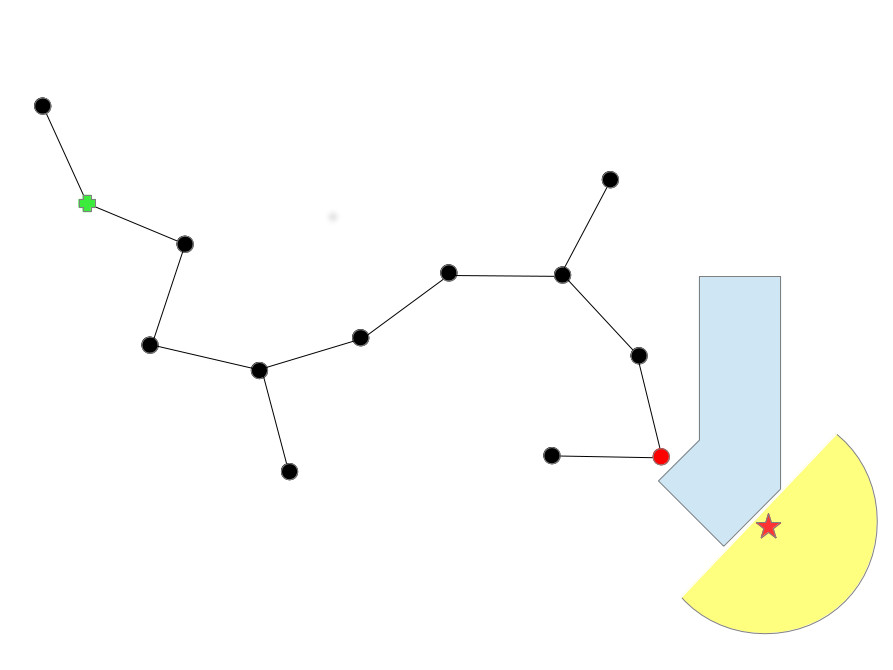
\includegraphics[width=0.5\textwidth]{figures/bugTrapRRT.jpg}
  \caption{An RRT attempting a bug trap problem. \label{fig:BugTrapRRT} }
\end{figure}

Figure ~\ref{fig:BugTrapRRT} shows an example of a single style RRT attempting to solve a problem where the goal is occluded by an object.
The state of the RRT is shown after 12 iterations of the extend operation. In this case, the probability of taking a step to goal was about
35\%. At this state we can see that two problems emerge in our quest to connect the tree to the goal node:
\begin{enumerate}
\item Future attempts to step to goal will be taken from the red node since it is closest. All these attempts will fail because there is an
obstacle in the way. Obviously, these attempts are a waste of time.
\item To actually get to the goal, the RRT will have to find its way into the yellow semicircle around the goal by virtue of only random
steps. Any nodes outside of this area will be either further than the red node or obstructed by the obstacle. The probability of this
happening quickly is very low. Essentially, it would require that random configurations to extend toward constantly be in the bottom right
corner of the workspace. In this case, the probability of getting such random configurations looks to be around 1/15. In a different
scenario with a larger workspace and smaller step size, this probability would be much smaller. 
\end{enumerate}

Some may argue that this problem occurs because the RRT is too greedy - that if the probability of stepping to goal was smaller, we would be
able to avoid the obstacle. This is not really the case. We can practically throw out the probability that the RRT will reach the goal
randomly, so we still need the tree to extend where a goal step would be useful. This is again a low probaility proposition if the goal is
near the edge of the workspaceand occluded by an obstacle. Moreover, less greedy RRTs naturally take longer to converge to goal in simpler
cases. In our opinion, the important takeaway is that fast RRTs generally tend to approach the goal in a very directed fashion.


\section{Forage RRT Implementation}

\section{Experiments and Evaluation}

\section{Discussion}

\bibliographystyle{plain}
\bibliography{RRT,MotionPlanning,IK}

\end{document}

